\documentclass{article}

\usepackage{amsmath, amsthm, amssymb, amsfonts}
\usepackage{thmtools}
\usepackage{graphicx}
\usepackage{setspace}
\usepackage{geometry}
\usepackage{float}
\usepackage[colorlinks=true, linkcolor=Blue]{hyperref}
\usepackage{cancel}
\usepackage[utf8]{inputenc}
\usepackage[english]{babel}
\usepackage{framed}
\usepackage[dvipsnames]{xcolor}
\usepackage{tcolorbox}
\usepackage{empheq}
\newtcolorbox{mymathbox}[1][]{colback=white, sharp corners, #1}
\usepackage{witharrows}

\author{Mauro Patimo}
\title{AERSP 508 Lecture 25}
\begin{document}
\maketitle
We can determine the drag coefficient by starting with the skin friction coefficient and integrating it over the surface of the body. Since the drag will be applied on both sides of the object, we need to multiply it by 2:
\begin{equation}
    C_D=\frac{2}{L}\int_0^L0.664\sqrt{\frac{\nu}{u_e}}x^{-\frac{1}{2}}dx
\end{equation}
where $u_e$ is the velocity at the end of the plate. The integral can be solved analytically and the result is:
\begin{equation}
    C_D=1.328\sqrt{\frac{\nu}{u_eL}}
\end{equation}
The Blasius profile is observed to approach the edge velocity asymptotically, so we cannot ascribe a definite thickness to the BL. However, we can define the boundary layer thickness as the distance from the wall where the velocity is 99\% of the edge velocity. This is also where $f'(\eta)=0.99$, which is $\eta=3.74$.
This gives 
\begin{equation}
    \delta=\delta_{99}=5.29\sqrt{\frac{\nu x}{u_e}}
\end{equation}
The Blasius similarity solution may be extended to flows over wedges, which are geometrically self-similar. The wedge angle is $\theta$ and the flow is assumed to be two-dimensional. The wedge is assumed to be semi-infinite, so the flow is assumed to be uniform at infinity. The velocity is $U_e=U_ox^m$. The angle of the wedge is $\pi\beta$. Beta is defined in the following way:
\begin{equation}
    \beta=\frac{2m}{1+m}
\end{equation}
$m$ can then be used to describe the angle of the wedge. We can find a relation between $m$ and the pressure gradient with Bernoulli's equation:
\begin{equation}
    \frac{1}{\rho}\frac{dP}{dx}=-U_e\frac{dU_e}{dx}=\frac{mU_e^2}{x} \footnote{$\frac{dU_e}{dx}=\frac{mU_e}{x}$ because $U_e=U_ox^m$}
\end{equation}
From this we can determine if the pressure gradient is favorable or adverse. If $m<0$, the pressure gradient is favorable, and if $m>0$, the pressure gradient is adverse. If $m=0$, the pressure gradient is zero. An example of a favorable pressure gradient is the flow encountering an obstacle, while an example of an adverse pressure gradient is a pipe increasing in diameter. As shown in Fig. \ref{fig:Wedges Examples}.
\begin{figure}
    \centering
    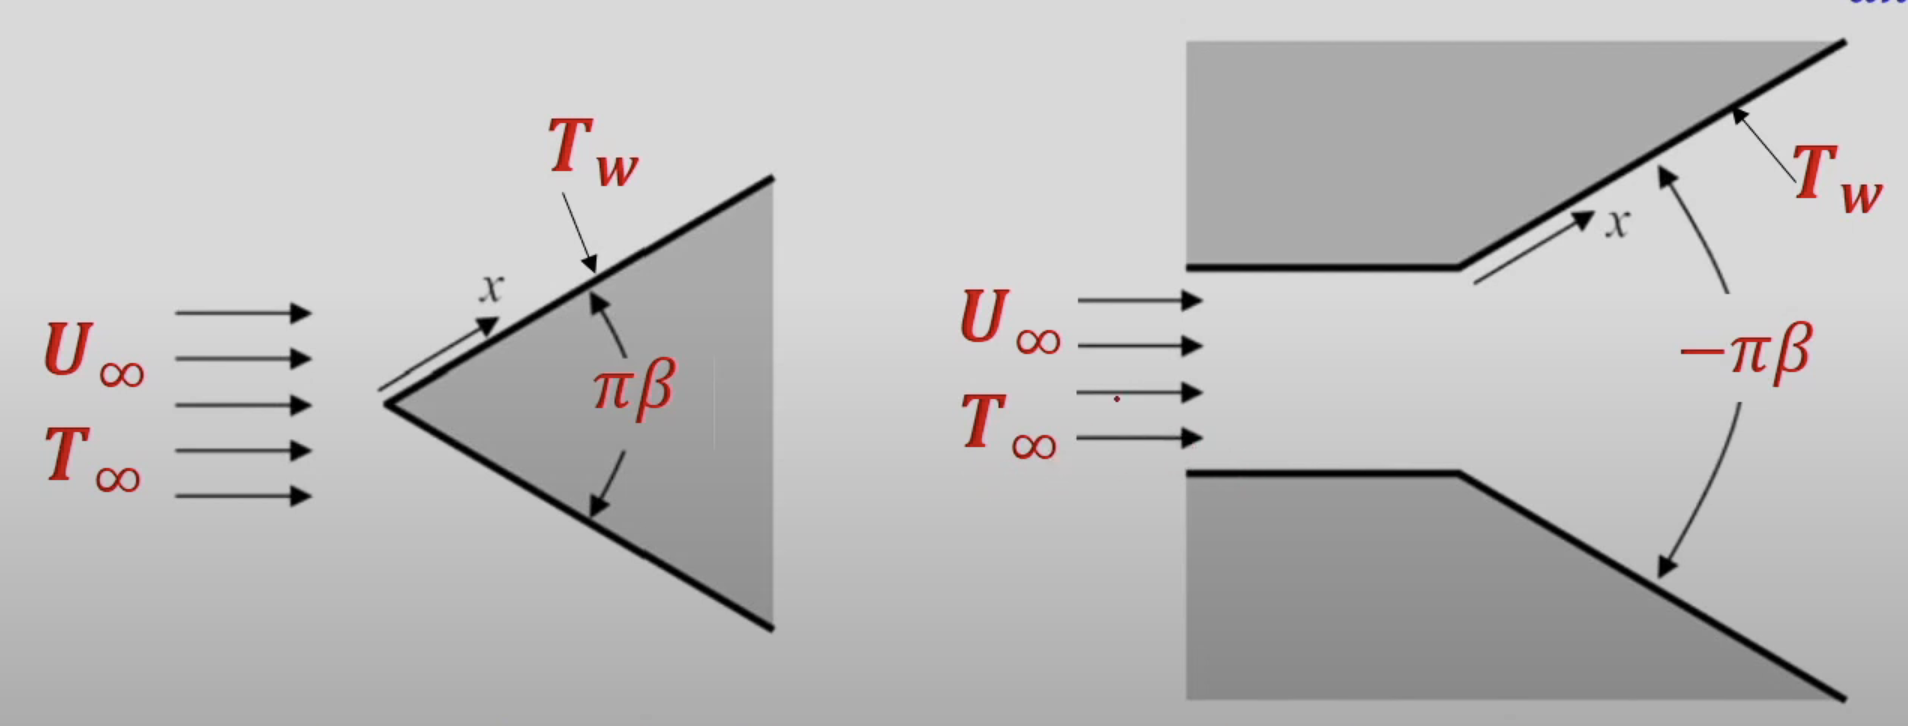
\includegraphics[width=\textwidth]{Wedges Examples.png}
    \caption{Examples of favorable and adverse pressure gradients. In this case $T$ stand for the temperature of the flow, but it is kept constant so it doesn't affect the flow.}
    \label{fig:Wedges Examples}
\end{figure}

Our variable $\eta$ is still defined as $\eta=\frac{y}{g(x)}$, but now $g(x)$ is defined as:
\begin{equation}
    g(x)=\sqrt{\frac{2\nu x}{U_e(1+m)}}
\end{equation}
And our $\psi$ is defined as:
\begin{equation}
    \psi=U_e(x)g(x)f(\eta)
\end{equation}
This gives us the following equations:
\begin{equation}
    f'''+ff''+\beta [1-f'^2]=0
\end{equation}
Also known as the Falkner-Skan equation. The boundary conditions are the same as before: $f(0)=f'(0)=0$ and $lim_{\eta \to \infty} f''(\eta)=1$.

Two notable solutions to this equation are $\beta$=0 (or when $m=0$), and when $\beta=1$ (or when $m=1$). The first value is the Blasius solution (or simply when the boundary is a flat plate). The second one instead is when there is a stagnation point flow. $f''(0)=0$ when $\beta=-0.19884$. \\

Other important properties about the flow are the momentum thickness $\theta$ and the displacement thickness $\delta^*$. We can derive them by model the bulk transport of a velocity deficit.:
\begin{align*}
    \frac{d}{dx}[u(U_e-e)]+\frac{d}{dy}[v(U_e-e)] & = \frac{1}{\rho}\frac{dP}{dx}-\nu \frac{d^2u}{dy^2}+\frac{d}{dx}(uU_e)+\frac{d}{dy}(vU_e) \\
\end{align*}
This can be written alternatively as:
\begin{align*}
    \frac{d}{dx}[u(U_e-e)]+\frac{d}{dy}[v(U_e-e)] & = -U_e\frac{dU_e}{dx}-\nu \frac{d^2u}{dy^2}+u\frac{dU_e}{dx}+U_e\frac{du}{dx}-U_e\frac{d^2u}{dy^2} \\
\end{align*}
The LHS of the equation is the advection of the velocity deficit, the term driving $U_e$ in terms of x is the pressure work, and the term with $\nu$ is the viscous work.\\
We rewrite the equation as:
\begin{align*}
    \frac{d}{dx}[u(U_e-e)]+\frac{d}{dy}[v(U_e-e)]+(U_e-u)\frac{dU_e}{dx}=-\nu\frac{d^u}{dy^2}
\end{align*}
To determine the bulk transport in the direction parallel to the surface, we integrate in the wall-normal direction:
\begin{align*}
    \int_0^{\delta} \frac{d}{dx}[u(U_e-e)]dy+\int_0^{\delta} \frac{d}{dy}[v(U_e-e)]dy+(U_e-u)\frac{dU_e}{dx}dy=-\nu\int_0^{\delta}\frac{d^u}{dy^2}dy
\end{align*}
The LHS of the equation is the bulk transport of the velocity deficit, while the RHS is the sum of the pressure gradient, the convection of the mean velocity, and the diffusion of the mean velocity. We can integrate the equation over the boundary layer thickness to get:
\begin{align*}
    \int_0^{\delta} \frac{d}{dx}[u(U_e-e)]dy+[v(U_e-u)]_0^\infty +\frac{dU_e}{dx}\int_0^\infty (U_e-u)dy & = \nu \frac{du}{dy}|_0^\infty\\
\end{align*}
The second term on the LHS is zero because $v=0$ at the wall and at infinity. The RHS is zero at infintiy, since $u$ is constant at infinity, but it is equal to $\frac{\tau}{\rho}$ at the wall.


\appendix
\section{Derivation of the Falkner-Skan equation}
Let's derive the equations we derived in the previous lectures, but for a non constant $U_e$.
\begin{align*}
    \psi & =U_e(x)g(x)f(\eta) \\
    u & =\frac{\partial\psi}{\partial y}=U_e(x)f'(\eta) \\
    v & =-\frac{\partial\psi}{\partial x}=U_e'(x)g(x)f(\eta)+U_e(x)g'(x)f(\eta)+U_e(x)\frac{g'(x)}{g^2(x)}f'(\eta) \\
\end{align*}

\begin{align*}
    \frac{\partial u}{\partial x}+\frac{\partial v}{\partial y} & =0 \\
    \frac{\partial u}{\partial x} & =U_e'(x)f'(\eta)+U_e(x)f''(\eta)\frac{\partial \eta}{\partial x} \\
    \frac{\partial v}{\partial y} & =U_e'(x)g(x)f'(\eta)+U_e(x)g'(x)f(\eta)+U_e(x)\frac{g'(x)}{g^2(x)}f'(\eta)\frac{\partial \eta}{\partial x} \\
    \frac{\partial \eta}{\partial x} & =\frac{y}{g(x)}\frac{\partial g(x)}{\partial x} \\
    \frac{\partial u}{\partial x}+\frac{\partial v}{\partial y} & =U_e'(x)f'(\eta)+U_e(x)f''(\eta)\frac{1}{g(x)}\frac{\partial g(x)}{\partial x}+U_e'(x)g(x)f'(\eta)+U_e(x)g'(x)f(\eta)+U_e(x)\frac{g'(x)}{g^2(x)}f'(\eta)\frac{1}{g(x)}\frac{\partial g(x)}{\partial x} \\
\end{align*}

\end{document}